\documentclass{standalone} % Utilise la classe standalone pour compiler uniquement le TikZ
%\include{pakage_tikz}
\usepackage{tikz}          % Charge le package TikZ
\usepackage{xcolor}        % Gestion avancée des couleurs
\usepackage{amsmath}       % Gestion des formules mathématiques
\usetikzlibrary{arrows.meta} % Pour gérer les flèches avec des formes spécifiées comme "triangle"
\usetikzlibrary {decorations.pathmorphing}
\usepackage{pgfplots}
\pgfplotsset{compat=1.18}
\usepackage[active,tightpage]{preview}
\PreviewEnvironment{tikzpicture}
\usetikzlibrary{arrows.meta}
\usetikzlibrary {arrows.meta,bending,positioning}
\usetikzlibrary {datavisualization.formats.functions}
%PREAMBULE pour schÃéma
\usepackage{pgfplots}
\usepackage{tikz}
\usepackage[european resistor, european voltage, european current]{circuitikz}
\usetikzlibrary{arrows,shapes,positioning}
\usetikzlibrary{decorations.markings,decorations.pathmorphing,
decorations.pathreplacing}
\usetikzlibrary{calc,patterns,shapes.geometric}
\usepackage{anyfontsize}
\usetikzlibrary{hobby, decorations.markings, arrows.meta}

\setlength\PreviewBorder{5pt}
%\usepgfplotslibrary{external}
%\tikzexternalize

%% Automatiser cela : une solution plus élégante  nouvelle page, tu peux utiliser la commande \newpage juste avant chaque \begin{tikzpicture}
%\let\oldtikzpicture\tikzpicture
%\let\endoldtikzpicture\endtikzpicture
%\renewenvironment{tikzpicture}{\newpage\oldtikzpicture}{\endoldtikzpicture}
%\usepackage{etoolbox} % dans le préambule, si pas encore utilisé
%\pretocmd{\tikzpicture}{\clearpage}{}{}


% Définition de la fonction pour générer la grille
\newcommand{\drawgrid}[4]{


	\begin{scope}[opacity = 0.2]
	
	
    	% Paramètres : #1=xmin, #2=xmax, #3=ymin, #4=ymax

   	 	% Grille principale en cm
    	\draw[very thin, gray] (#1,#3) grid (#2,#4); % Grille de base (1 cm)
    
    	\draw[very thin, gray] (#1,#3) grid[step=0.1] (#2,#4);

    	\draw[thin, black] (#1,#3) edge[thick,line width=0.8ex,->,>=Stealth ] (#2,#3); 
    
    	\foreach \x in {#1,..., #2} {
        	\draw[shift={(\x, #3)}] (0,-0.1) edge[line width=0.8ex] node[pos = -1 , below] {\x} (0,0.1); % Lignes verticales en mm
    	}

    	\draw[thin, black] (#1,#3)edge[thick,line width=0.8ex,->,>=Stealth ] (#1,#4); 
    
    	\foreach \y in {#3,..., #4} {
        	\draw[shift={(#1, \y)}] (-0.1 , 0 ) edge[line width=0.8ex] node[pos = -1 , left ] {\y} (0.1 , 0); % Lignes verticales en mm
    	}
    
    \end{scope}


}


\newcommand{\Axex}[1][$x$]{ % "x" est la valeur par défaut de #1
    \draw
        (-10, 0) edge[thick, line width=0.8ex, ->, >=Triangle, color=\colorThree] 
        node[shift = {(0,1)} , pos=1.01, below]{ \huge #1 } (10, 0)
        ;
}

\newcommand{\Axetheta}[1][$\theta$]{
	\draw
		(-10, 0 ) edge [thick,line width=0.8ex,->,>=Triangle , color = \colorThree ]node [pos=1.01,right]{\huge #1 } ( 10  , 0 )
	;
}

\newcommand{\Axedensity}[1][$n$]{
	\draw
		(0, -1 ) edge [thick,line width=0.8ex,->,>=Triangle , color = \colorThree ]node [pos=1.01,left  ]{\huge #1 } ( 0  , 6 )
	;
}

\newcommand{\Axedistribution}[1][$\nu$]{
	\draw
		(0, -1 ) edge [thick,line width=0.8ex,->,>=Triangle , color = \colorThree ]node [pos=1.01,left  ]{\huge #1 } ( 0  , 6 )
	;
}

\newcommand{\Axesphase}[2][$x$]{
	\Axex[#1]
	\begin{scope}[rotate = 90]
		\Axetheta[#2]	
	\end{scope}
}

\newcommand{\Axesdensity}[2][$x$]{
	\Axex[#1]
	\Axedensity[#2]
}

\newcommand{\Axesdistribution}[2][\theta]{
	\Axetheta[#1]
	\Axedistribution[#2]
}

\newcommand{\Axetemps}[1][Deformation]{
	\draw 
		(-5 , 0 ) edge [line width=2.8ex, color=\colorOne ]( 0, 0)
		(43 , 0 ) edge [line width=2.8ex, color=\colorOne , ->, >=Triangle] node[pos = 1.0 , right , scale = 2 ] { \fontsize{60pt}{720pt}\selectfont $\tilde{t}$} ( 50 , 0)
		( 0 , 1 ) edge [line width=2.0ex, color=\colorOne ] ( 0 , -1 )  
		( 43 , 1 ) edge [line width=2.0ex, color=\colorOne ] ( 43 , -1 ) 
		(0 , 0) edge[<->, > = stealth, line width=2.8ex, color=\colorOne ]  node [ rectangle , midway, fill = white , scale = 2 ] {\fontsize{600pt}{720pt}\selectfont \bf  #1}(43, 0)  
	;

}

\newcommand{\Palette}[1][\colorOne]{
	\clip[decorate, decoration={random steps, segment length=3pt, amplitude=3pt}]
        	(-1,-1) rectangle (1,1);
	\draw[fill=#1 , color = #1 ] (-2,-2) rectangle (2,2);
}






% Définition des couleurs avec les codes HTML
\definecolor{colorOne}{HTML}{443E46}
%\definecolor{colorTwo}{HTML}{F6DEB8}
\definecolor{colorTwo}{HTML}{FFFFFF}

\definecolor{colorThree}{HTML}{908CA4}
\definecolor{colorFour}{HTML}{57659E}
\definecolor{colorFive}{HTML}{C57284}
\definecolor{colorSix}{HTML}{FF5B69}

% Raccourcis pour les couleurs
\def\colorOne{colorOne}
\def\colorTwo{colorTwo}
\def\colorThree{colorThree}
\def\colorFour{colorFour}
\def\colorFive{colorFive}
\def\colorSix{colorSix}
\definecolor{colorGold}{HTML}{FFD700}
\def\colorGold{colorGold}



% Graduation ordonné
	
\newcommand{\GraduationYMm}[2]{
	\foreach \r in {1,...,9} {
		\draw 
			({-0.25 * 0.5 * (cos(3.14*0.2*\r r)^2 + 1)}, #1*#2 - #2 + 0.1*#2*\r) 
			edge [thick, line width=0.3ex, color=\colorOne] 
			({0.25 * 0.5 * (cos(3.14*0.2*\r r)^2 + 1)}, #1*#2 - #2 + 0.1*#2*\r);
	}
}

\newcommand{\GraduationYCm}[4]{% #1: min, #2: max, #3: liste
  \foreach \R in {#1,...,#2} {
    \pgfmathparse{#3[\R-(#1)]} % index dans la liste
    \let\labelText\pgfmathresult

    \draw[color=\colorThree]
      (-0.3, \R*#4)
      edge [thick, line width=0.5ex, color=\colorOne]
      node [pos=-0.0, left]{\Large \labelText}
      (0.3, \R*#4);

    %\GraduationYMm{\R}{#4}
  }

  % Graduation supplémentaire à #2 + 3
  \pgfmathparse{#2 + 1}
  \edef\extendedPosition{\pgfmathresult}
  %\GraduationYMm{\extendedPosition}{#4}
}

\newcommand{\GraduationXMm}[2]{
	\foreach \r in {1,...,9} {
		\draw 
			( #1*#2 - #2 + 0.1*#2*\r,{-0.25 * 0.5 * (cos(3.14*0.2*\r r)^2 + 1)}) 
			edge [thick, line width=0.3ex, color=\colorOne] 
			( #1*#2 - #2 + 0.1*#2*\r,{0.25 * 0.5 * (cos(3.14*0.2*\r r)^2 + 1)});
	}
}

\newcommand{\GraduationXCm}[4]{% #1: min, #2: max, #3: liste
  \foreach \R in {#1,...,#2} {
    \pgfmathparse{#3[\R-(#1)]} % index dans la liste
    \let\labelText\pgfmathresult

    \draw[color=\colorThree]
      (\R*#4,-0.3)
      edge [thick, line width=0.5ex, color=\colorOne]
      node [pos=-0.0, below]{\Large \labelText}
      (\R*#4,0.3);

    %\GraduationXMm{\R}{#4}
  }

  % Graduation supplémentaire à #2 + 3
  \pgfmathparse{#2 + 1}
  \edef\extendedPosition{\pgfmathresult}
  %\GraduationXMm{\extendedPosition}{#4}
}

% Définition de la fonction pour générer la grille
\newcommand{\backgrowngrid}[6]{


	\begin{scope}[xscale = #5 , yscale = #6 ]
	
	
    	% Paramètres : #1=xmin, #3=xmax, #2=ymin, #4=ymax
    	%\clip[scale = 0.95 , decorate, decoration={random steps, segment length=0.1 cm, amplitude=0.2cm}](#1 , #2 ) rectangle ( #3 , #4 ) ;
    	\pgfmathparse{#1-1}  
    	\let\valXmin\pgfmathresult
    	\pgfmathparse{#2-1}  
    	\let\valYmin\pgfmathresult
    	\pgfmathparse{#3+1}  
    	\let\valXmax\pgfmathresult
    	\pgfmathparse{#4+1}  
    	\let\valYmax\pgfmathresult
    	
    	\draw[fill = \colorThree , opacity = 0.1]  (\valXmin , \valYmin ) rectangle ( \valXmax , \valYmax ) ;

   	 	% Grille principale en cm
    	\draw[very thin, line width=0.5ex ,  color=\colorTwo] (\valXmin , \valYmin ) grid ( \valXmax , \valYmax ); % Grille de base (#5 cm , #6 cm )
    
    	%\draw[very thin, line width=0.3ex ,  color=\colorTwo] (#1,#2) grid[step=0.1] (#3,#4);

    	%\draw[thin, black] (#1,#2) edge[thick,line width=0.8ex,->,>=Stealth ] (#3,#2); 
    
    	%\foreach \x in {#1,..., #3} {
    	%	\pgfmathparse{int(\x * #5)} % calcule et arrondit \pgfmathparse{round((\x * #5)/10)*10} Par exemple, au multiple de 10 le plus proche 
    	%	\let\val\pgfmathresult
        %	\draw[shift={(\x, #2)}] (0,-0.1) edge[line width=0.8ex] node[pos = -1 , below] {\val} (0,0.1); % Lignes verticales en mm
    	%}

    	%\draw[thin, black] (#1,#2)edge[thick,line width=0.8ex,->,>=Stealth ] (#1,#4); 
    
    	%\foreach \y in {#2,..., #4} {
    	%	\pgfmathparse{int(\y * #6)} % calcule et arrondit  
    	%	\let\val\pgfmathresult
        %	\draw[shift={(#1, \y)}] (-0.1 , 0 ) edge[line width=0.8ex] node[pos = -1 , left ] {\val} (0.1 , 0); % Lignes verticales en mm
    	%}
    
    \end{scope}


}



\begin{document}


\begin{tikzpicture}[use Hobby shortcut]
           
	%\fill[fill=\colorFour , decoration={random steps,segment length=2mm} , decorate , closed] (-1,-1) -- (-1,11) --(11,11) -- (11,-1)-- cycle ;
    %\fill[fill=\colorFour ] (0,0) -- (0,10)  -- (10,0) ;
	
        
	\begin{scope}[shift={(4.5,5)} , scale = 1.3]
		%\draw[fill= black ] (-5,-5) rectangle + (10 , 10) ;
  		\newcommand{\curve}{(-2,-1) .. (1,-2) .. (2,2) .. (0,1)} 

		\foreach \i in {0,...,49} { % 50 couches
    		\pgfmathsetmacro{\s}{1.5 - 0.015*\i}
    		\pgfmathsetmacro{\c}{2*\i}   % mélange de 0% à 98%
    		\draw[closed, scale=\s, fill=colorSix!\c!colorTwo, draw=none] \curve -- cycle;
		}

		\begin{scope}[shift={(-4.5,1)} , scale = 1.0]
			\draw[fill=\colorFour , opacity = 0.5 , draw = none  ]
				(1.9,0) rectangle (9.85, 0.5 )
			;
			\draw[line width=0.5ex, color=\colorFour , dashed]
				(2,0) -- (9.75,0)
				(2,0.5) -- (9.75,0.5)
			;
			\draw[color=\colorFour]
				(10,0) edge[<->, line width=0.1ex , ultra thick] node[pos= 0.5 , right]{\fontsize{20pt}{16pt}\selectfont $\delta \theta$} (10,0.5)
			;
			\begin{scope}%[overlay]
				\node[] (point) at (4,0.1) {};
	        	\draw[  opacity = 1 ]
		        	(point) edge[line width=0.4ex ,color = \colorFour ,arrows = {Computer Modern Rightarrow[sharp ,length=0.2cm]-} , out = 90 , in = 180  ]node[pos=1, right , font = \fontsize{12pt}{16pt}\selectfont]{\color{colorFour} \fontsize{20}{10}\selectfont \bfseries \begin{tabular}{c} $\displaystyle \int dx \rho ( x , \theta ; t ) \, \delta \theta = \Pi(\theta) \, \delta \theta  $  \\[0.2cm] \textbf{is conserved} \end{tabular} }($(point) + (2.0cm,2.0cm)$)
             	;
        	\end{scope}
		\end{scope}
    
	\end{scope}

	\node[draw = none , fill=none, minimum width=3cm, minimum height=2cm, align=center, \colorTwo] 
        at (5,4) {\fontsize{20pt}{16pt}\selectfont $\rho(x , \theta ; t )$};
	%\node[draw = none , fill=none, minimum width=3cm, minimum height=2cm, align=center, \colorTwo] 
    %    at (8,1.5) {\fontsize{20pt}{16pt}\selectfont $\nu = 0 $};

    % \node[draw = none , fill=none, minimum width=3cm, minimum height=2cm, align=center , \colorTwo , rotate = 40] 
    %     at (5,4.5) {\fontsize{20pt}{16pt}\selectfont $\nu = 1$};
    


   
%    \draw[ ]
%    		%(8,6.5) edge[line width=0.3ex, color=\colorThree , dashed ] node [pos = 0 , below ,\colorThree ]{\fontsize{10pt}{16pt}\selectfont $x_2$} (8,9)
%    		%(8,7.25) edge[line width=0.3ex, color=\colorThree , ->] node [pos = 1 , below ,\colorThree ]{\fontsize{10pt}{16pt}\selectfont $v^{\mathrm{eff}}_{[\rho ]}(\theta_+)$}(9,7.25) 
%    		(3,1.5) edge[line width=0.5ex, color=\colorGold!50!\colorThree , dashed ] node [pos = 0 , below ,\colorGold!50!\colorThree]{\fontsize{15pt}{16pt}\selectfont $x_1$}(3,6)
%    		(3,5.4) edge[line width=0.5ex, color=\colorGold!50!\colorThree , ->] node [pos = 1 , below ,\colorGold!50!\colorThree]{\fontsize{15pt}{16pt}\selectfont $v^{\mathrm{eff}}_{[\rho  ]}(\theta_-)$}(2.0,5.4) 
%    ;
          
    
    
    
    % Axe horizontal (gamma)
    \draw[ line width=0.8ex, color=\colorOne , ->] 
        (-0.5,0) -- (10.5,0) 
        node[shift = {(0,0)} , pos=0.5, below] {\fontsize{20pt}{19pt}\selectfont $x$};

    % Axe vertical (t)
    \draw[ line width=0.8ex, color=\colorOne , ->] 
        (0,-0.5) -- (0,10.5) 
        node[ shift = {(0,0)} , pos=0.5, above, rotate=90] {\fontsize{20pt}{19pt}\selectfont $\theta$};
        
    
        
    %\drawgrid{-2}{10}{-1}{10};
\end{tikzpicture}

% \AtBeginDocument{\shorthandoff{:;!?}}
% \tikzset{every picture/.style={execute at begin picture={\shorthandoff{:;!?};}}}
% \tikzstyle{every picture}+=[remember picture]
% \tikzstyle{na} = [shape=rectangle,inner sep=0pt]


% \newcommand{\ptFleche}[2]{		% Déclaration d'une extrémité de flèche
%     \shorthandoff{:;!?}% <- désactive les shorthands
%     \tikz[baseline=(#1.base)]\node[na](#1){#2};
% }

\begin{tikzpicture}

	\node[] at (0,0) {
		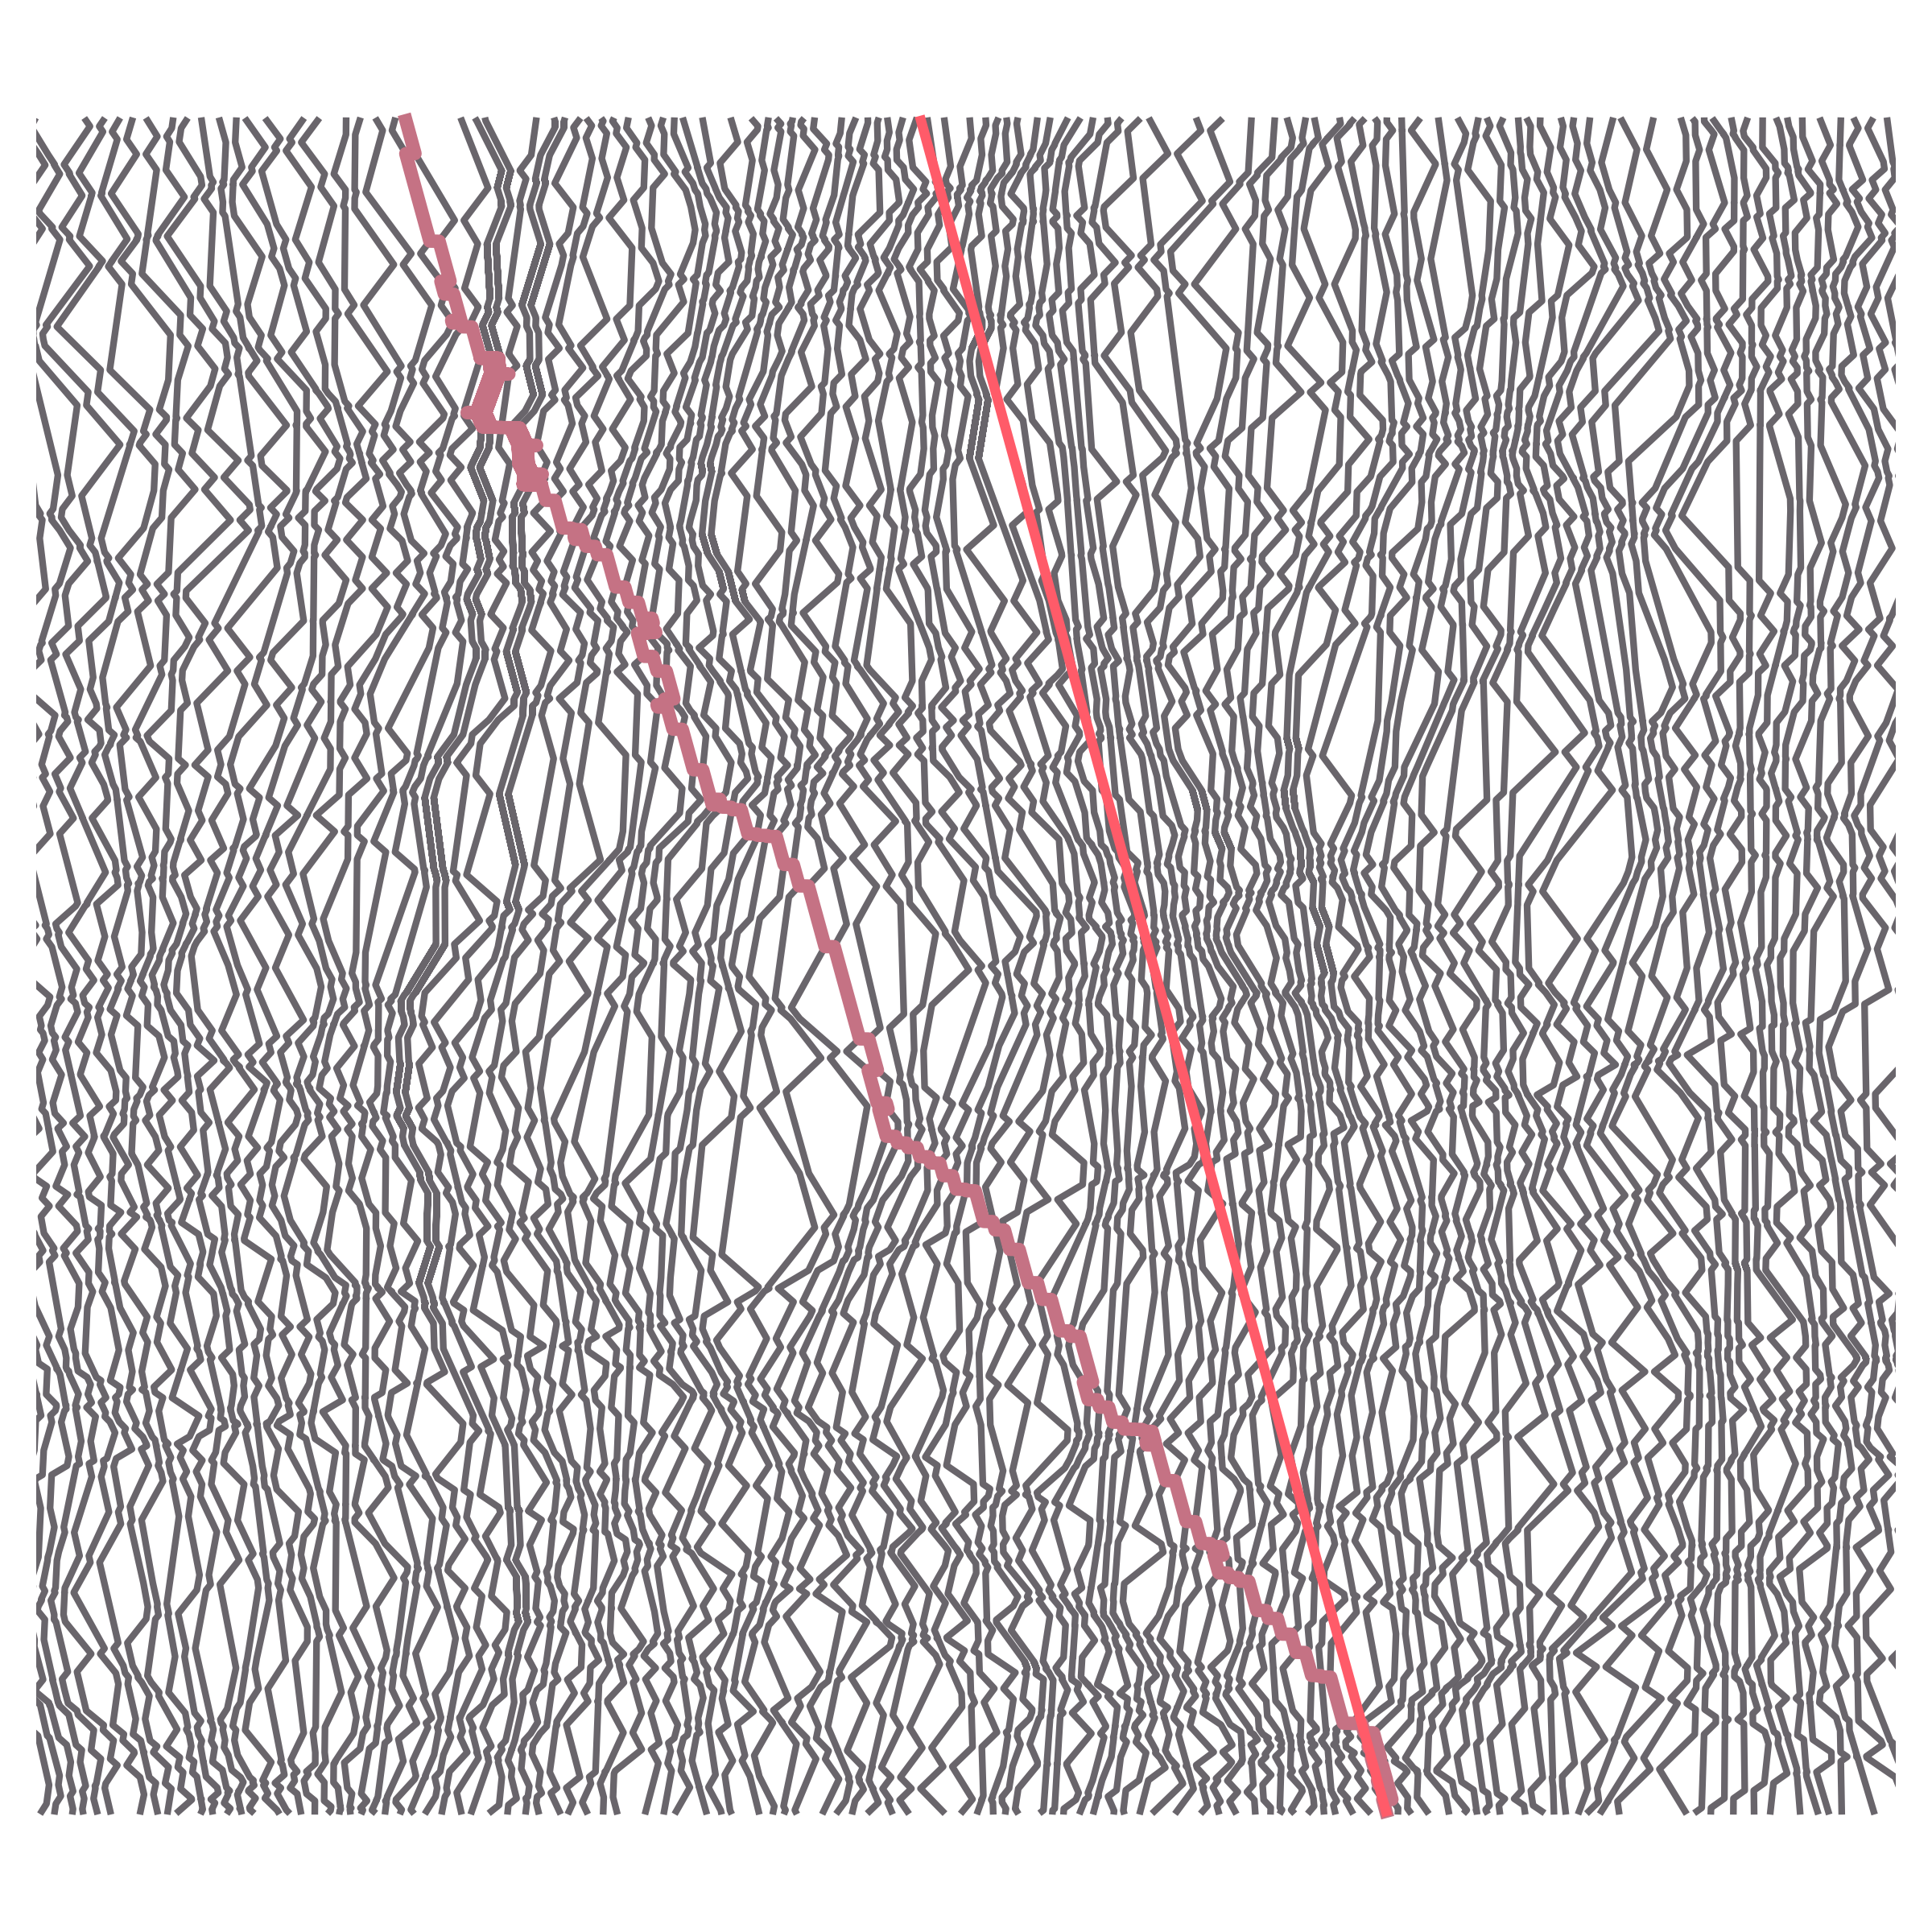
\includegraphics[width=1.0\textwidth]{trajectoires_hard_rods.png}
	};

	% Axxes 
	\draw[shift = {(-6.0,-5.5)}]
		(-1, 0) edge[thick, line width=0.5ex, ->, color=\colorOne] node[shift = {(0,0)} , pos=0.5, below]{\fontsize{22pt}{16pt}\selectfont  \color{\colorOne} position } (12, 0)
		(-0, -1) edge[thick, line width=0.5ex, ->, color=\colorOne] node[shift = {(0,0)} , pos=0.5, above , rotate = 90 ]{\fontsize{22pt}{16pt}\selectfont\color{\colorOne} time } (-0, 11)		
	;

	\node (pointveff) at (-3.5,5.2) {};
	\node (pointve)   at (-0.2,5.2) {};

	\draw[ opacity = 1.0 ]

	    (pointveff) edge[line width=0.4ex ,color = colorFive ,arrows = {Computer Modern Rightarrow[sharp ,length=0.2cm]-},  , out = 90 , in = 180  ]node[pos=1, right]{\color{colorFive} \fontsize{15}{10}\selectfont \bfseries  $ \displaystyle  v^{\mathrm{eff}}_{[\rho]}(v)  $ }($(pointveff) + (1cm,0.75cm)$)

        (pointve) edge[line width=0.4ex ,color = colorSix ,arrows = {Computer Modern Rightarrow[sharp ,length=0.2cm]-},  , out = 90 , in = 180  ]node[pos=1, right]{\color{colorSix} \fontsize{15}{10}\selectfont \bfseries  $ \displaystyle  v $ }($(pointve) + (1cm,0.75cm)$)

		% (motDelta) edge[line width=0.4ex ,color = colorSix ,arrows = {Computer Modern Rightarrow[sharp ,length=0.2cm]-},  , out = 90 , in = 0  ]node[pos=1, left]{\color{colorSix} \fontsize{10}{10}\selectfont \bfseries  - diameters of balls }($(motDelta) + (-1cm,1.0cm)$)

		% (motcolli) edge[line width=0.4ex ,color = colorSix ,arrows = {Computer Modern Rightarrow[sharp ,length=0.2cm]-},  , out = -150 , in = 150  ]node[pos=1, right]{\color{colorSix} \fontsize{10}{10}\selectfont \bfseries  number of collisions per second }($(motcolli) + (-1cm,-1.0cm)$)


	;

	%\drawgrid{-7}{7}{-7}{7}

\end{tikzpicture}

\begin{tikzpicture}[use Hobby shortcut]
    
        
    % Rectangle avec texte "Tonks Girardeau"
    
        
    %\fill[fill=\colorFour , decoration={random steps,segment length=2mm} , decorate ] (1,1) -- (0,10) --(10,10) -- (10,0) ;
    %\fill[fill=\colorFour ] (0,0) -- (0,10)  -- (10,0) ;
    \node[draw = none , fill=none, minimum width=3cm, minimum height=2cm, align=center, \colorThree] 
        at (2.5,9) {\fontsize{20pt}{16pt}\selectfont $\nu_{[\rho]}(x , \theta ; t )$};
    \node[draw = none , fill=none, minimum width=3cm, minimum height=2cm, align=center, \colorThree] 
        at (8,1.5) {\fontsize{20pt}{16pt}\selectfont $\nu = 0 $};
        
%    \fill[fill=\colorSix] 
%    plot[smooth cycle] coordinates {
%    	(2,2)
%        (4,8)
%        (7,9)
%        (8.5,6)
%        (8,4)
%        (5.5,3)        
%        %(3.5,4)
%        %(4,5)
%    };

	\begin{scope}[shift={(4.5,5)} , scale = 1.3]
	%\draw[fill= black ] (-5,-5) rectangle + (10 , 10) ;
  \newcommand{\curve}{(-2,-1) .. (1,-2) .. (2,2) .. (0,1)} 

  % Remplissage
  \fill[shift={(0,0)}, \colorSix, closed] \curve -- cycle;

  % Partie 0–40% : dashed en colorTwo + label
  
  \begin{scope}
  	\clip (-5,-3) -- (5,3) -- (-5, 5 ) -- cycle;
  	\draw[shift={(0,0)}, postaction={decorate}, 
        decoration={markings,
          mark=at position 0.2 with   {
            \node[sloped, pos = 0.5 , above , \colorFour ]{\fontsize{14pt}{16pt}\selectfont \bf{$\theta_-(x,t)$}} ;
          },
          reverse path,
        }]
    [closed, dashed, ultra thick,line width=1.0ex, color=\colorFour] \curve -- cycle;
	
	
	%\fill[white , opacity = 0.5](-5,-5) -- (5,4) -- (-5, 5 ) -- cycle ;
	\end{scope}
  	\begin{scope}
  		\clip (-5,-3) -- (5,3) -- (5, -5 ) -- cycle;
  		\draw[shift={(0,0)}, postaction={decorate}, 
        decoration={markings,
          mark=at position 0.6 with   {
            \node[sloped, pos = 0.5 , above , \colorOne!50!\colorTwo ]{\fontsize{14pt}{16pt}\selectfont \bf{$\theta_+(x,t)$}} ;
          },
          reverse path,
        }]
    [closed, dashed, ultra thick,line width=1.0ex, color=\colorOne!50!\colorTwo] \curve -- cycle;
    %\fill[white , opacity = 0.5](-5,-5) -- (5,4) -- (5, -5 ) -- cycle ;
    \end{scope}
    
    \end{scope}


    \node[draw = none , fill=none, minimum width=3cm, minimum height=2cm, align=center , \colorTwo , rotate = 40] 
        at (5,4.5) {\fontsize{20pt}{16pt}\selectfont \bf{$\nu = 1$}};
    

   
   \draw[ ]
   		%(8,6.5) edge[line width=0.3ex, color=\colorThree , dashed ] node [pos = 0 , below ,\colorThree ]{\fontsize{10pt}{16pt}\selectfont $x_2$} (8,9)
   		%(8,7.25) edge[line width=0.3ex, color=\colorThree , ->] node [pos = 1 , below ,\colorThree ]{\fontsize{10pt}{16pt}\selectfont $v^{\mathrm{eff}}_{[\rho ]}(\theta_+)$}(9,7.25) 
   		(3,1.5) edge[line width=0.8ex, color=\colorGold!50!\colorThree , dashed ] node [pos = 0 , below ,\colorGold!50!\colorThree]{\fontsize{15pt}{16pt}\selectfont \bf{$x_1$}}(3,6)
   		(3,5.4) edge[line width=0.8ex, color=\colorGold!10!\colorThree , ->] node [pos = 1 , left ,\colorGold!10!\colorThree]{\fontsize{15pt}{16pt}\selectfont \bf{$v^{\mathrm{eff}}_{[\rho  ]}(\theta_-)$}}(2.0,5.4) 
   ;
          
    
    
    
    % Axe horizontal (gamma)
    \draw[ line width=0.8ex, color=\colorOne , ->] 
        (-0.2,0) -- (10.5,0) 
        node[shift = {(0,0)} , pos=0.5, below] {\fontsize{20pt}{19pt}\selectfont $x$};

    % Axe vertical (t)
    \draw[ line width=0.8ex, color=\colorOne , ->] 
        (0,-0.2) -- (0,10.5) 
        node[ shift = {(0,0)} , pos=0.5, above, rotate=90] {\fontsize{20pt}{19pt}\selectfont $\theta$};
        
    
        
    %\drawgrid{-2}{10}{-1}{10};
\end{tikzpicture}



\begin{tikzpicture}
    
        
    % Rectangle avec texte "Tonks Girardeau"
    
        
    \fill[fill=\colorFour , decoration={random steps,segment length=2mm} , decorate ] (1,1) -- (0,10) --(10,10) -- (10,0) ;
    \fill[fill=\colorFour ] (0,0) -- (0,10)  -- (10,0) ;
    \node[draw = none , fill=none, minimum width=3cm, minimum height=2cm, align=center, \colorTwo] 
        at (2,9) {\fontsize{10pt}{16pt}\selectfont $\nu_{[\rho]}(x , \theta ; t )$};
    \node[draw = none , fill=none, minimum width=3cm, minimum height=2cm, align=center, \colorTwo] 
        at (7,2) {\fontsize{10pt}{16pt}\selectfont $\nu = 0 $};
        
    \fill[fill=\colorSix] (1,1.5) -- (6.5,8.5) -- (9,8.5) -- (3.5,1.5) ;
    \node[draw = none , fill=none, minimum width=3cm, minimum height=2cm, align=center , \colorTwo , rotate = 50] 
        at (5,5) {\fontsize{10pt}{16pt}\selectfont $\nu = 1$};
       
        
   \draw[ ]
   		(1,1.5) edge [line width=0.6ex, color=\colorGold , dashed ] node[sloped, pos = 0.5 , above , \colorGold ]{\fontsize{10pt}{16pt}\selectfont $\theta_-(x,t)$} (6.5,8.5) 
   		(6.5,8.5) edge [line width=0.4ex, color=\colorGold , dashed ] (9,8.5) 
   ; 
   \draw[ ]
   		(1,1.5) edge[line width=0.6ex, color=\colorTwo , dashed ] (3.5,1.5)
   		(3.5,1.5) edge[line width=0.4ex, color=\colorTwo , dashed ] node[sloped, pos = 0.5 ,below , \colorTwo ]{\fontsize{10pt}{16pt}\selectfont $\theta_+(x,t)$} (9,8.5)  
   ;
   
   \draw[ ]
   		(8,6.5) edge[line width=0.3ex, color=\colorThree , dashed ] node [pos = 0 , below ,\colorThree ]{\fontsize{10pt}{16pt}\selectfont $x_2$} (8,9)
   		(8,7.25) edge[line width=0.3ex, color=\colorThree , ->] node [pos = 1 , below ,\colorThree ]{\fontsize{10pt}{16pt}\selectfont $v^{\mathrm{eff}}_{[\rho ]}(\theta_+)$}(9,7.25) 
   		(2.5,1) edge[line width=0.3ex, color=\colorThree , dashed ] node [pos = 0 , below ,\colorThree ]{\fontsize{10pt}{16pt}\selectfont $x_1$}(2.5,4)
   		(2.5,3.4) edge[line width=0.3ex, color=\colorThree , ->] node [pos = 1 , below ,\colorThree]{\fontsize{10pt}{16pt}\selectfont $v^{\mathrm{eff}}_{[\rho  ]}(\theta_-)$}(1.5,3.4) 
   ;
          
    
    
    
    % Axe horizontal (gamma)
    \draw[ line width=0.8ex, color=\colorOne , ->] 
        (-0.2,0) -- (10.5,0) 
        node[shift = {(0,0)} , pos=0.5, below] {\fontsize{16pt}{19pt}\selectfont $x$};

    % Axe vertical (t)
    \draw[ line width=0.8ex, color=\colorOne , ->] 
        (0,-0.2) -- (0,10.5) 
        node[ shift = {(0,0)} , pos=0.5, above, rotate=90] {\fontsize{16pt}{19pt}\selectfont $\theta$};
        
    
        
    %\drawgrid{-2}{10}{-1}{10};
\end{tikzpicture}


\begin{tikzpicture}[use Hobby shortcut]
    
        
    % Rectangle avec texte "Tonks Girardeau"
    
        
    \fill[fill=\colorFour , decoration={random steps,segment length=2mm} , decorate ] (1,1) -- (0,10) --(10,10) -- (10,0) ;
    \fill[fill=\colorFour ] (0,0) -- (0,10)  -- (10,0) ;
    \node[draw = none , fill=none, minimum width=3cm, minimum height=2cm, align=center, \colorTwo] 
        at (2.5,9) {\fontsize{20pt}{16pt}\selectfont $\nu_{[\rho]}(x , \theta ; t )$};
    \node[draw = none , fill=none, minimum width=3cm, minimum height=2cm, align=center, \colorTwo] 
        at (8,1.5) {\fontsize{20pt}{16pt}\selectfont $\nu = 0 $};
        
%    \fill[fill=\colorSix] 
%    plot[smooth cycle] coordinates {
%    	(2,2)
%        (4,8)
%        (7,9)
%        (8.5,6)
%        (8,4)
%        (5.5,3)        
%        %(3.5,4)
%        %(4,5)
%    };

	\begin{scope}[shift={(4.5,5)} , scale = 1.3]
	%\draw[fill= black ] (-5,-5) rectangle + (10 , 10) ;
  \newcommand{\curve}{(-2,-1) .. (1,-2) .. (2,2) .. (0,1)} 

  % Remplissage
  \fill[shift={(0,0)}, \colorSix, closed] \curve -- cycle;

  % Partie 0–40% : dashed en colorTwo + label
  
  \begin{scope}
  	\clip (-5,-3) -- (5,3) -- (-5, 5 ) -- cycle;
  	\draw[shift={(0,0)}, postaction={decorate}, 
        decoration={markings,
          mark=at position 0.2 with   {
            \node[sloped, pos = 0.5 , above , \colorGold ]{\fontsize{12pt}{16pt}\selectfont $\theta_-(x,t)$} ;
          },
          reverse path,
        }]
    [closed, dashed, ultra thick,line width=0.6ex, color=\colorGold] \curve -- cycle;
	
	
	%\fill[white , opacity = 0.5](-5,-5) -- (5,4) -- (-5, 5 ) -- cycle ;
	\end{scope}
  	\begin{scope}
  		\clip (-5,-3) -- (5,3) -- (5, -5 ) -- cycle;
  		\draw[shift={(0,0)}, postaction={decorate}, 
        decoration={markings,
          mark=at position 0.6 with   {
            \node[sloped, pos = 0.5 , above , \colorTwo ]{\fontsize{12pt}{16pt}\selectfont $\theta_+(x,t)$} ;
          },
          reverse path,
        }]
    [closed, dashed, ultra thick,line width=0.6ex, color=\colorTwo] \curve -- cycle;
    %\fill[white , opacity = 0.5](-5,-5) -- (5,4) -- (5, -5 ) -- cycle ;
    \end{scope}
    
    \end{scope}


    \node[draw = none , fill=none, minimum width=3cm, minimum height=2cm, align=center , \colorTwo , rotate = 40] 
        at (5,4.5) {\fontsize{20pt}{16pt}\selectfont $\nu = 1$};
    
    %\newcommand{\curve}{(-2,-1) .. (1,-2) .. (2,2) .. (0,1)}    
    % Remplissage de la patate
	%\fill[\colorSix , shift = {(5,5)} , closed] 
	%\curve -- cycle;
%   	(3,3) .. controls (2.5,6) and (5,8.5) .. (7,9)
%           .. controls (8,8) and (9,6.5) .. (8.5,4.5)
%           .. controls (7.5,3) and (6,2.5) .. (5.5,3)
%           .. controls (4.5,2.5) and (3.5,2.5) .. (3,3);
           
       
    %\fill[closed,\colorSix,] \curve;
    
    % Remplissage de la forme
%\fill[\colorSix] \curve -- cycle;

% Contour de 0 à 40% en or pointillé


%% Contour de 40% à 100% en gris pointillé
%\draw[, shift = {(5,5)} , closed ,dashed, ultra thick, %color=\colorTwo,
%      postaction={decorate,
%        decoration={show path construction,
%          lineto code={
%            \draw[dashed, ultra thick, color=\colorTwo] (\tikzinputsegmentfirst) edge[dashed, ultra thick, color=\colorTwo] node[sloped, pos = 0.5 ,below , \colorTwo ]{\fontsize{10pt}{16pt}\selectfont $\theta_+(x,t)$} (\tikzinputsegmentlast);
%          }
%        }
%      }]
%  \curve -- cycle;
%  
%  \draw[, shift = {(5,5)} , closed ,dashed, ultra thick, %color=\colorTwo,
%      postaction={decorate,
%        decoration={show path construction,
%          %lineto code={
%          mark=between positions 0 and 0.4 step 1 with {
%            \draw[dashed, ultra thick, color=\colorTwo] (\tikzinputsegmentfirst) edge[dashed, ultra thick, color=\colorTwo] node[sloped, pos = 0.5 ,below , \colorTwo ]{\fontsize{10pt}{16pt}\selectfont $\theta_+(x,t)$} (\tikzinputsegmentlast);
%          }
%        }
%      }]
%  \curve -- cycle;
  
%  decoration={markings,
%    mark=between positions 0 and 0.4 step 1 with {
%      \draw[dashed, ultra thick, \colorTwo] 
%        (\tikzinputsegmentfirst) -- (\tikzinputsegmentlast);
%           
%% Partie gauche (θ_-)
%\draw[
%    dashed, thick, color=\colorGold, line width=0.6ex,
%    decoration={markings,
%        mark=at position 0.5 with {
%            \node[sloped, above, font=\fontsize{10pt}{16pt}\selectfont, color=\colorGold] {$\theta_-(x,t)$};
%        }
%    },
%    postaction=decorate
%] 
%    (3,3) .. controls (3.5,6) and (5,8.5) .. (7,9);
%
%% Partie droite (θ_+)
%\draw[
%    dashed, thick, color=\colorTwo, line width=0.6ex,
%    decoration={markings,
%        mark=at position 0.5 with {
%            \node[sloped, above, line width=0.6ex, font=\fontsize{10pt}{16pt}\selectfont, color=\colorTwo] {$\theta_+(x,t)$};
%        }
%    },
%    postaction=decorate
%]
%    (7,9) .. controls (8,8) and (9,6.5) .. (8.5,4.5)
%           .. controls (7.5,3) and (6,2.5) .. (5.5,3)
%           .. controls (4.5,2.5) and (3.5,2.5) .. (3,3);
%
%   

   
   \draw[ ]
   		%(8,6.5) edge[line width=0.3ex, color=\colorThree , dashed ] node [pos = 0 , below ,\colorThree ]{\fontsize{10pt}{16pt}\selectfont $x_2$} (8,9)
   		%(8,7.25) edge[line width=0.3ex, color=\colorThree , ->] node [pos = 1 , below ,\colorThree ]{\fontsize{10pt}{16pt}\selectfont $v^{\mathrm{eff}}_{[\rho ]}(\theta_+)$}(9,7.25) 
   		(3,1.5) edge[line width=0.5ex, color=\colorGold!50!\colorThree , dashed ] node [pos = 0 , below ,\colorGold!50!\colorThree]{\fontsize{15pt}{16pt}\selectfont $x_1$}(3,6)
   		(3,5.4) edge[line width=0.5ex, color=\colorGold!50!\colorThree , ->] node [pos = 1 , below ,\colorGold!50!\colorThree]{\fontsize{15pt}{16pt}\selectfont $v^{\mathrm{eff}}_{[\rho  ]}(\theta_-)$}(2.0,5.4) 
   ;
          
    
    
    
    % Axe horizontal (gamma)
    \draw[ line width=0.8ex, color=\colorOne , ->] 
        (-0.2,0) -- (10.5,0) 
        node[shift = {(0,0)} , pos=0.5, below] {\fontsize{20pt}{19pt}\selectfont $x$};

    % Axe vertical (t)
    \draw[ line width=0.8ex, color=\colorOne , ->] 
        (0,-0.2) -- (0,10.5) 
        node[ shift = {(0,0)} , pos=0.5, above, rotate=90] {\fontsize{20pt}{19pt}\selectfont $\theta$};
        
    
        
    %\drawgrid{-2}{10}{-1}{10};
\end{tikzpicture}



\begin{tikzpicture}[scale=0.8,
  decoration={markings,
    mark=between positions 0.25 and 0.25 step 0.5
    with {\node[sloped,above,scale=0.9] {$\theta_-(x,t)$};},
    mark=between positions 0.75 and 0.75 step 0.5
    with {\node[sloped,below,scale=0.9] {$\theta_+(x,t)$};}
  }]

% La patate remplie
\fill[\colorSix]
    plot[smooth cycle] coordinates {
        (2,2)
        (4,8)
        (7,9)
        (8.5,6)
        (8,4)
        (5.5,3)
    };

% Contour moitié en or pointillé
\draw[postaction=decorate, dashed, ultra thick, color=\colorGold]
    plot[smooth,tension=1] coordinates {
        (2,2)
        (4,8)
        (7,9)
        (8.5,6)
    };

% Contour moitié en gris pointillé
\draw[postaction=decorate, dashed, ultra thick, color=\colorTwo]
    plot[smooth,tension=1] coordinates {
        (8.5,6)
        (8,4)
        (5.5,3)
        (2,2)
    };

\end{tikzpicture}




\begin{tikzpicture}[use Hobby shortcut]
\newcommand{\curve}{(-2,-1) .. (1,-2) .. (2,2) .. (0,1)}
\draw[
closed,
decoration={
  markings,
  mark=at position 0.2 with {\draw[red, thick, -Stealth] (0,0) -- (0.6,0); \draw[thick, -Stealth] (0,0) -- (0,0.6);},
  mark=at position 0.3 with {\draw[red, thick, -Stealth] (0,0) -- (0.6,0); \draw[thick, -Stealth] (0,0) -- (0,0.6);},
  mark=at position 0.7 with {\draw[red, thick, -Stealth] (0,0) -- (0.6,0); \draw[thick, -Stealth] (0,0) -- (0,0.6);},
 },  
postaction={decorate},
] \curve;
\draw[closed, scale=0.8] \curve;
\draw[closed, scale=0.6] \curve;
\draw[closed, scale=0.4] \curve;
\end{tikzpicture}


\begin{tikzpicture}[use Hobby shortcut]


	\draw[fill= black ] (-5,-5) rectangle + (10 , 10) ;
  \newcommand{\curve}{(-2,-1) .. (1,-2) .. (2,2) .. (0,1)} 

  % Remplissage
  \fill[shift={(0,0)}, \colorSix, closed] \curve -- cycle;

  % Partie 0–40% : dashed en colorTwo + label
  
  \begin{scope}
  	\clip (-5,-5) -- (5,4) -- (-5, 5 ) -- cycle;
  	\draw[shift={(0,0)}, postaction={decorate}, 
        decoration={markings,
          mark=at position 0.2 with   {
            \node[sloped, pos = 0.5 , above , \colorGold ]{\fontsize{12pt}{16pt}\selectfont $\theta_-(x,t)$} ;
          },
          reverse path,
        }]
    [closed, dashed, ultra thick,line width=0.6ex, color=\colorGold] \curve -- cycle;
	
	
	%\fill[white , opacity = 0.5](-5,-5) -- (5,4) -- (-5, 5 ) -- cycle ;
	\end{scope}
  	\begin{scope}
  		\clip (-5,-5) -- (5,4) -- (5, -5 ) -- cycle;
  		\draw[shift={(0,0)}, postaction={decorate}, 
        decoration={markings,
          mark=at position 0.6 with   {
            \node[sloped, pos = 0.5 , above , \colorTwo ]{\fontsize{12pt}{16pt}\selectfont $\theta_+(x,t)$} ;
          },
          reverse path,
        }]
    [closed, dashed, ultra thick,line width=0.6ex, color=\colorTwo] \curve -- cycle;
    %\fill[white , opacity = 0.5](-5,-5) -- (5,4) -- (5, -5 ) -- cycle ;
    \end{scope}

\end{tikzpicture}


\begin{tikzpicture}[use Hobby shortcut]

  % Définition de la courbe fermée (patate)
  \def\curve{(-2,-1) .. (1,-2) .. (2,2) .. (0,1) -- cycle}

  % Remplissage
  \fill[shift={(5,5)}, \colorSix , closed] \curve;

  % Première moitié : θ_-(x,t), couleur Gold
  \draw[shift={(5,5)}, dashed, ultra thick, \colorGold, postaction={decorate},
        decoration={markings, mark=at position 0.2 with {
            \node[sloped, above, \colorGold, font=\fontsize{10pt}{16pt}\selectfont]{$\theta_-(x,t)$};
        }}]
    (-2,-1) .. (1,-2) .. (2,2);

  % Deuxième moitié : θ_+(x,t), couleur Two
  \draw[shift={(5,5)}, dashed, ultra thick, \colorTwo, postaction={decorate},
        decoration={markings, mark=at position 0.6 with {
            \node[sloped, above, \colorTwo, font=\fontsize{10pt}{16pt}\selectfont]{$\theta_+(x,t)$};
        }}]
    (2,2) .. (0,1) .. (-2,-1);

\end{tikzpicture}





\end{document}
